\documentclass[a4paper,11pt]{article}
% My own packages
\usepackage{amsmath, amsthm, amssymb} %For advanced math
\usepackage{graphicx} %Graphics
\usepackage{float} %Floating Graphics
\usepackage{enumerate} %Enumerate
\usepackage{lipsum} % Package to generate dummy text throughout this template
\usepackage[sc]{mathpazo} % Use the Palatino font
\usepackage[T1]{fontenc} % Use 8-bit encoding that has 256 glyphs
\linespread{1.05} % Line spacing - Palatino needs more space between lines
\usepackage{microtype} % Slightly tweak font spacing for aesthetics
\usepackage[margin={2cm,3cm},hmarginratio=1:1,top=32mm,columnsep=20pt]{geometry} % Document margins
\usepackage{multicol, framed} % Used for the two-column layout of the document
\usepackage{hyperref} % For hyperlinks in the PDF
\usepackage[hang, small,labelfont=bf,up,textfont=it,up]{caption} % Custom captions under/above floats in tables or figures
\usepackage{booktabs} % Horizontal rules in tables
\usepackage{lettrine} % The lettrine is the first enlarged letter at the beginning of the text
\usepackage{paralist} % Used for the compactitem environment which makes bullet points with less space between them
\usepackage{abstract} % Allows abstract customization
\renewcommand{\abstractnamefont}{\normalfont\bfseries} % Set the "Abstract" text to bold
\renewcommand{\abstracttextfont}{\normalfont\small\itshape} % Set the abstract itself to small italic text
\usepackage{minted}
\usepackage{fancyhdr} % Headers and footers
\pagestyle{fancy} % All pages have headers and footers
\fancyhead{} % Blank out the default header
\fancyfoot{} % Blank out the default footer
\fancyhead[L]{CS 5220 Final Project} % Custom header text
\fancyfoot[RO,LE]{\thepage} % Custom footer text

%----------------------------------------------------------------------------------------
%	TITLE SECTION
%----------------------------------------------------------------------------------------

\title{\vspace{-15mm}\fontsize{24pt}{10pt}\selectfont\textbf{CS 5220 Final Project \\ \Large Alternating Direction Implicit}} % Article title
\author{
\large
\textsc{Batu Inal [bi49], Bob(Kunhe) Chen [kc853]}\\
\normalsize Cornell University \\ % Your institution
[2mm] 
\vspace{-20mm}
}
\date{}
%----------------------------------------------------------------------------------------
\begin{document}
\setlength{\textwidth}{500pt}
\maketitle % Insert title
\thispagestyle{fancy} % All pages have headers and footers
%----------------------------------------------------------------------------------------
%	ABSTRACT
%----------------------------------------------------------------------------------------
\begin{abstract}
\noindent %Abstract
For our final project, we studied the Alternating Direction Implicit method that was proposed by Douglas Jr. in 1953. We started from a C++ reference code and later rewrote it in C for finer control over memory access and vectorization. We did algorithmetic improvement over the original code to get further performance boost. We report our results of optimizing the serial and parallel code for our final implementation of the Douglas ADI method.
%% Change Title and Fancy Head Parts first !!
\end{abstract}
%----------------------------------------------------------------------------------------
%	ARTICLE CONTENTS
%----------------------------------------------------------------------------------------
\begin{multicols}{2}
\section{Alternating Direction Implicit}
	\subsection{Application}
	Alternating direction implicit (ADI) is an iterative method for solving multidimensional partial differential equations(PDEs) using finite difference method. The ADI method is most used to solve parabolic equations on rectangular domains, such as heat conduction and diffusion equations in two dimensions and above. An alternative solver for heat conduction equation is Crank-Nicolson method, which is implicit in time and  unconditionally stable.  Crank-Nicolson method inverts a matrix at each time step and it soon becomes clumsy when the problem size keeps increasing. The ADI method, instead of solving the two-dimensional problem, solves a succession of many one-dimensional problems, while retaining the ability to stay stable unconditionally. It is also noteworthy that the ADI method can be easily extended to solve 3D problems, although the unconditional stability no longer holds.
	\subsection{Algorithm}
	Given a heat conduction equation with boundary condition,
	\[div({\bf a}({\bf x})\nabla{\bf u}) = {\bf f},\quad {\bf x}\in\Omega\]
	\[{\bf u}({\bf x}) = {\bf g}({\bf x}),\quad \forall {\bf x}\in\partial \Omega\]
	The central idea of the ADI method is to obtain a solution by evolving
	\[\frac{\partial \tilde{\bf u}}{\partial t} = div({\bf a}({\bf x})\nabla\tilde{\bf u}) - {\bf f}\]
	to a steady state, i.e., when $||\frac{\partial \tilde{u}}{\partial t}||_2 = 0$. For simplicity of our discussion, we assume $\bf a$ to be constant along one direction (in 2D). The ADI method approximate the process using:
	\[({\bf I} - \frac{dt}{2}\alpha_x\Delta_x){\bf u}_{k+1}^* = ({\bf I}+\frac{dt}{2}\alpha_x\Delta{\bf x}+dt\alpha_y\Delta y){\bf u}_k - dt {\bf f}\]
	\[({\bf I} - \frac{dt}{2}\alpha_y\Delta_y){\bf u}_{k+1} = {\bf u}_{k+1}^*-\frac{dt}{2}\alpha_y\Delta_y{\bf u}_k\]
The ADI method solves the 2D problem first in the $x$ direction and then in the $y$ direction, thus giving rise to the name Alternating Direction.
\par There are two matrix-vector multiplications and two backsolve in each iteration. For the matrix-vector multiplication, it consists the sum of difference operators and identity matrices. The difference operator approximates differential on a finite grid:
	\[\Delta_x {\bf u} = (u_{i+1}-u_{i-1})/2\Delta x\]
	so the linear system is tridiagonal. Similarly, we will backsolve a tridiagonal linear system twice to get the final answer.
\par Given a tridiagonal system, we have fast algorithms to compute them directly. For matrix-vector multiplication, a naive implementation will work because it is not computationally intense enough for further optimization. For backsolving tridiagonal system, we use Thomas algorithm.
\par For a tridiagonal square matrix,
\[\bf Ax = b\] 
Thomas algorithm first computes the LU factorization
\[\bf LUx = b\]
and then it solves the problem sequentially
\[\bf Ux = L^{-1}b\]
\[\bf x = U^{-1}L^{-1}b\]
The matrices $\bf L$ and $\bf U$ have only one sub/super-diagonal because they are factorized from a tridiagonal one. The two backsolve can be done easily using one \texttt{for} loop to iterate through their sub/super-diagonal elements.
\par For the final implementation, we have
\begin{enumerate}
\item Apply forward operator $\Delta_x$ to $\bf u$.
\item Apply forward operator $\Delta_y$ to $\bf u$.
\item Sum the results up and subtract $dt{\bf f}$.
\item Backsolve the problem in the $x$ direction.
\item Subtract $\frac{dt}{2}\alpha_y\Delta_y {\bf u}_k$ from the result.
\item Backsolve the problem in the $y$ direction.
\end{enumerate}
	\subsection{Convergence}
	\par The relaxation of 
	\[\frac{\partial \tilde{\bf u}}{\partial t} = div({\bf a}({\bf x})\nabla\tilde{\bf u}) - {\bf f}\]
	gaurantees to converge to the actual solution. If we look at the error between ${\bf u(x,}t)$ and exact solution $\bf u(x)$, 
	\[\tilde{\bf e} = {\bf u(x,} t) - {\bf u(x)}\]
	Insert this into the relaxation equation:
	\[\frac{\partial }{\partial t}(\tilde{\bf u} - {\bf u}) = div({\bf a}({\bf x})\nabla(\tilde{\bf u}-{\bf u}))\]
	\[\Rightarrow \frac{\partial }{\partial t} {\tilde{\bf e}} = div({\bf a}({\bf x})\nabla\tilde{\bf e})\]
	Examine the following equation:
	\[\frac{1}{2}\int_{\Omega} \tilde{\bf e}\frac{\partial \tilde{\bf e}}{\partial t}d{\bf x} = \frac{1}{2}\int_{\Omega}\tilde{\bf e}div({\bf a}({\bf x})\nabla\tilde{\bf e})d{\bf x}\]
	Note that our boundary condition is fixed and so we have $\tilde{e} \equiv 0$ $\forall {\bf x} \in\partial\Omega$. Then we can apply the divergence theorem ($div(\rho{\bf w}) = \rho div({\bf w}) + \nabla \rho\cdot {\bf w}$) to get:
	\[\frac{1}{2}\int_{\Omega}\frac{\partial^2 \tilde{\bf e}}{\partial t^2}d{\bf x} = -\frac{1}{2}\int_{\Omega}{\bf a}({\bf x})(\nabla\tilde{\bf e})^2d{\bf x}\]
	Write it using norm:
	\[\frac{1}{2}\frac{d}{dt}\int_{\Omega}||\tilde{\bf e}||_2^2d{\bf x} = -\frac{1}{2}\int_{\Omega}{\bf a}({\bf x})|\nabla\tilde{\bf e}|^2d{\bf x} < 0\]
	So the derivative of the error norm $||\tilde{\bf e}||_2^2$ is strictly decreasing and therefore will converge to $0$.
	\par Although the convergence is gauranteed, an implementation that uses fixed timestep can easily take up to $10,000$ steps before the error becomes acceptable. One important idea from Douglas' paper is that the algorithm will use variable timesteps to speed up the convergence. If we look at the value of ${\bf u}$ as a sum of Fourier modes, each mode will converge at different rate for each timestep. So we will sweep through different timesteps to ensure all modes will converge more evenly. We determine the range of timesteps to take based on the size of our domain (which will limit the possible Fourier modes).
\section{Implementation}
	\subsection{C code} We started our work from a reference implementation of the Douglas ADI method using C++. We used this code both as a starting point to optimize the implementation of the algorithm, and later as a reference to check the correctness of our results.
\par The C++ code performs well when handling general problems, but it is not as easy for us to fine tune it for Totient. Therefore, we decided to rewrite it in C and apply techniques that we ahve learned in this course.
\par One challenge is to determine the data structure we will use. Because Douglas ADI method performs linear operations in both x and y directions, there does not exist one unique data structure that we can use to avoid striding across the data array. We decided to store the original data columnwise because most of the operations can be done in x direction. We perform a matrix transpose before applying the y-backsolver so that we can take advantage of spatial locality of the data. As in matrix multiplication project, the cost to transpose a matrix before carrying out the operation is compensated by the speedup from better data access.
\par We also tried to use \texttt{float} instead of \texttt{double} data type for faster computation. However, because each ADI iteration only stops when the difference between two consecutive matrices is smaller than our threshold $\varepsilon$ (in our case, it is set to be $10^{-6}$), we ended up taking many more steps than before and losing performance as a result. In the end, we kept using double as our data type throughout the program.
\section{Optimization}
	\subsection{Bottleneck}
	We used Intel Amplifier to find the bottleneck in our code. In both of the C++ and C code, the performance bottleneck is applying backsolve operators in the $x$ and $y$ directions. A sample report from initial stage of the optimization looks like:
\end{multicols}
\begin{minipage}{\textwidth}
	\begin{framed}
		\begin{center}
			\begin{verbatim}
Function                    Module       CPU Time  Spin Time  Overhead Time
--------------------------  -----------  --------  ---------  -------------
solve_tri_special           douglas-adi    0.804s         0s             0s
relaxOperation              douglas-adi    0.408s         0s             0s
[Outside any known module]  [Unknown]      0.254s         0s             0s
__intel_ssse3_rep_memcpy    douglas-adi    0.193s         0s             0s
transpose                   douglas-adi    0.121s         0s             0s
apply_tri_special           douglas-adi    0.020s         0s             0s
apply_tri_special_plus      douglas-adi    0.016s         0s             0s
main                        douglas-adi    0.013s         0s             0s
__svml_cos4                 douglas-adi    0.001s         0s             0s
__svml_cos4_l9              douglas-adi    0.001s         0s             0s
normInf                     douglas-adi    0.001s         0s             0s
			\end{verbatim}	
		\end{center}
	\end{framed}
\end{minipage}
\begin{multicols}{2}
	 It is not surprising that the backsolver takes most of the time since it is more expensive to compute at each step. It is noteworthy, however, the backsolver takes less than 50\% of the total computation time. The function \verb|relaxOperation()| alone takes approximately half as long to compute and all it does is adding and subtracting matrix values.
\par The result is likely caused by a cache miss in our naive attempt to implement the calculation using a single \verb|for| loop.
	\subsection{Cache Friendly Operations}
	In the original code, we have operations like
	\begin{minted}{c}
for (int i = 0; i < n*n; i++) {
	ustar[i] -= 0.5*u_t[i];
}
	\end{minted}
	We examined the individual function using the Intel Amplifier and observed that it the for loop took much longer than it should. So we created new functions to optimize their cache memory usage by using blocks. We modified a cache efficient matrix transpose program for our purpose and made it work:
\end{multicols}
\begin{minipage}{\textwidth}
\begin{minted}{c}
void transpose_cache(double* restrict dst,const double* restrict src, size_t n){
    __assume_aligned(dst, 64);
    __assume_aligned(src, 64);
    size_t block=64;
    for(size_t i = 0; i < n-block; i += block)
        for(size_t j=0; j < n; ++j ){
            for(size_t b = 0; b < block ; ++b){
                dst[j*n+b]=src[b*n+j];
            }
        }
    size_t start = n - n%block;
    for(size_t j=0; j < n; ++j )
        for(size_t b = start; b < n; ++b){
            dst[j*n+b]=src[b*n+j];
        }
}	
\end{minted}
\end{minipage}
\vspace{1mm}
\par
In addition to matrix tranpose, the function is also modified to carry out (2D) vector subtract, addition and transposed addition. After the change, the new report looks like
\\
\noindent \begin{minipage}{\textwidth}
	\begin{framed}
		\begin{center}
			\begin{verbatim}
Function                    Module                     CPU Time 
--------------------------  -------------------------  -------- 
solve_tri_special           douglas-adi                  0.990s                                              
[Outside any known module]  [Unknown]                    0.276s                                              
__intel_ssse3_rep_memcpy    douglas-adi                  0.119s                                              
vec_transpose_add           douglas-adi                  0.085s                                               
transpose_cache             douglas-adi                  0.056s                                              
vec_subtract                douglas-adi                  0.054s                                              
vec_subtract_half           douglas-adi                  0.052s                                              
apply_tri_special_plus      douglas-adi                  0.036s                                              
main                        douglas-adi                  0.023s                                              
apply_tri_special           douglas-adi                  0.021s                                              
__svml_cos4_l9              douglas-adi                  0.003s                                              
malloc                      libc-2.12.so                 0.003s                                              
_int_free                   libc-2.12.so                 0.002s                                              
normInf_cache               douglas-adi                  0.002s                                              
			\end{verbatim}	
		\end{center}
	\end{framed}
\end{minipage}
\begin{multicols}{2}
The hotspots reports don't necessarily reflect the exact behavior of the program, because the second one is running OpenMP with only $1$ threads (it will slow down the serial code), but we can see qualitatively that the most computation is now concentrated at the backsolver.
	\subsection{Vectorization}
	For vectorization, we largely reply on the compiler to do the work. We used \verb|_mm_malloc| to tell intel compiler to assign aligned memory blocks so that our calculation can be vectorized. Correspondingly, we used \verb|_mm_free()| to free the memory after using them.
	\par We tried to allocate scratch space for intermediate steps, but it didn't not work in our favor. When we allocated scratch space for backsolvers, they showed little contribution to the overall speed. However, as we started parallelization, they greatly reduced the speed of program, so we decided to allocate memory space in the function as they do not seem to be the limiting factor of our computation speed.
	\par In addition to that, we experimented with different compiler flags to get better performance for the code. In the end, we decided to use the following set of flags:
	\begin{center}
	\begin{verbatim}
	-O3 -no-prec-div -xcore -ansi-alias \
	-opt-prefetch -ftree-vectorize \
	-vec-threshold0 -ip
	\end{verbatim}
	\end{center}
	\subsection{Other changes}
	We here report some other changes that brought performance to our code.
	\par In the original code, we calculate the difference norm between two iterations only after one complete sweep ($dt_0\rightarrow dt_{max} \rightarrow dt_0$), since the calculating the norm and saving/updating the matrix from last step ${\bf u}_{k-1}$ is expensive. For a problem of size $2000$-by-$2000$, it takes about 72 iterations for the problem to converge and that is three timestep sweeps. If we look back at the cost of \verb|memcpy| and \verb|normInf|, we can check the difference norm more frequently and stop the iteration earlier.
	\par We do one more difference norm calculation halfway through the time sweep and check if we can stop then. For $2000$-by-$2000$ case, we can stop the problem at 60 iterations, thus saving us the cost to compute the extra steps.
	\par The other improvement we have is that we do not explicitly form the tridiagonal matrix in question. Instead, we compute them on the fly based on the parameter we are given for the problem. This way, we do not have to use extra memory space to save the matrix, and there is little redundant computation since most of the computation does not take much work. We increased the arithematic intensity of our code by eliminating the use of unnecessary memory space. 
	\subsection{OpenMP and Load Balancing}
    We use OpenMP for parallel computation of our code. Because it is costly to enter an OpenMP section, we have to use it sparingly. After experimenting with different strategy, it turns out that the only section that worths any parallelization is the backsolving part. The parallelization is easy in the sense that we are solving a series of independent linear system in 1D. However, we have to transpose the matrix ${\bf u}_k$ and subtract $\frac{dt}{2}\alpha_y\Delta_y {\bf u}_k$ from it, which makes a barrier between the two backsolvers indispensable.
    \par In a naive implementation of OpenMP, we are faced with enormous wait time in the hotspots report. This is probably because the solution ${\bf u}_k$ has a highly non-uniform distribution across the 2D space. As a result, a static scheduling will cause hugh load imbalance and thus slowing down our program. We tried different scheduling for the OpenMP (static, guided and dynamic). In the end, we chose to use \verb|schedule(dynamic,8)| because it yields the best performance.
\section{Performance}
	\subsection{Comparison with Reference Code}
	\end{multicols}
	\begin{table}[H]
	\centering
	\label{my-label}
	\begin{tabular}{lllllllllllll}
	Size(N)  & 200    & 400    & 800   & 1200  & 1600  & 2000  & 2400  & 2800  & 3200  & 3600  & 4000  \\ \cline{1-12}
	C        & 0.1449 & 0.5322 & 2.115 & 4.473 & 6.676 & 10.39 & 16.27 & 22.57 & 29.46 & 36.89 & 46.46 \\ 
	C++      & 0.1339 & 0.6365 & 3.178 & 8.178 & 14.84 & 23.62 & 40.87 & 50.11 & 72.63 & 91.71 & 113.9 \\
	C(16p)   & 0.3035 & 0.3445 & 1.092 & 1.663 & 2.262 & 3.972 & 5.780 & 8.012 & 9.979 & 13.75 & 16.55 \\
	C++(16p) & 0.0579 & 0.2355 & 1.156 & 2.642 & 4.806 & 7.618 & 11.91 & 16.39 & 20.90 & 30.75 & 33.30 \\
	\end{tabular}
	\caption{Scalability test for C and C++ code. The performance is measured by how much time (s) it takes to run problem of fixed size (N). Both serial and parallel codes are tested.}
	\end{table}
	
	\begin{figure}[H]
        \centering
                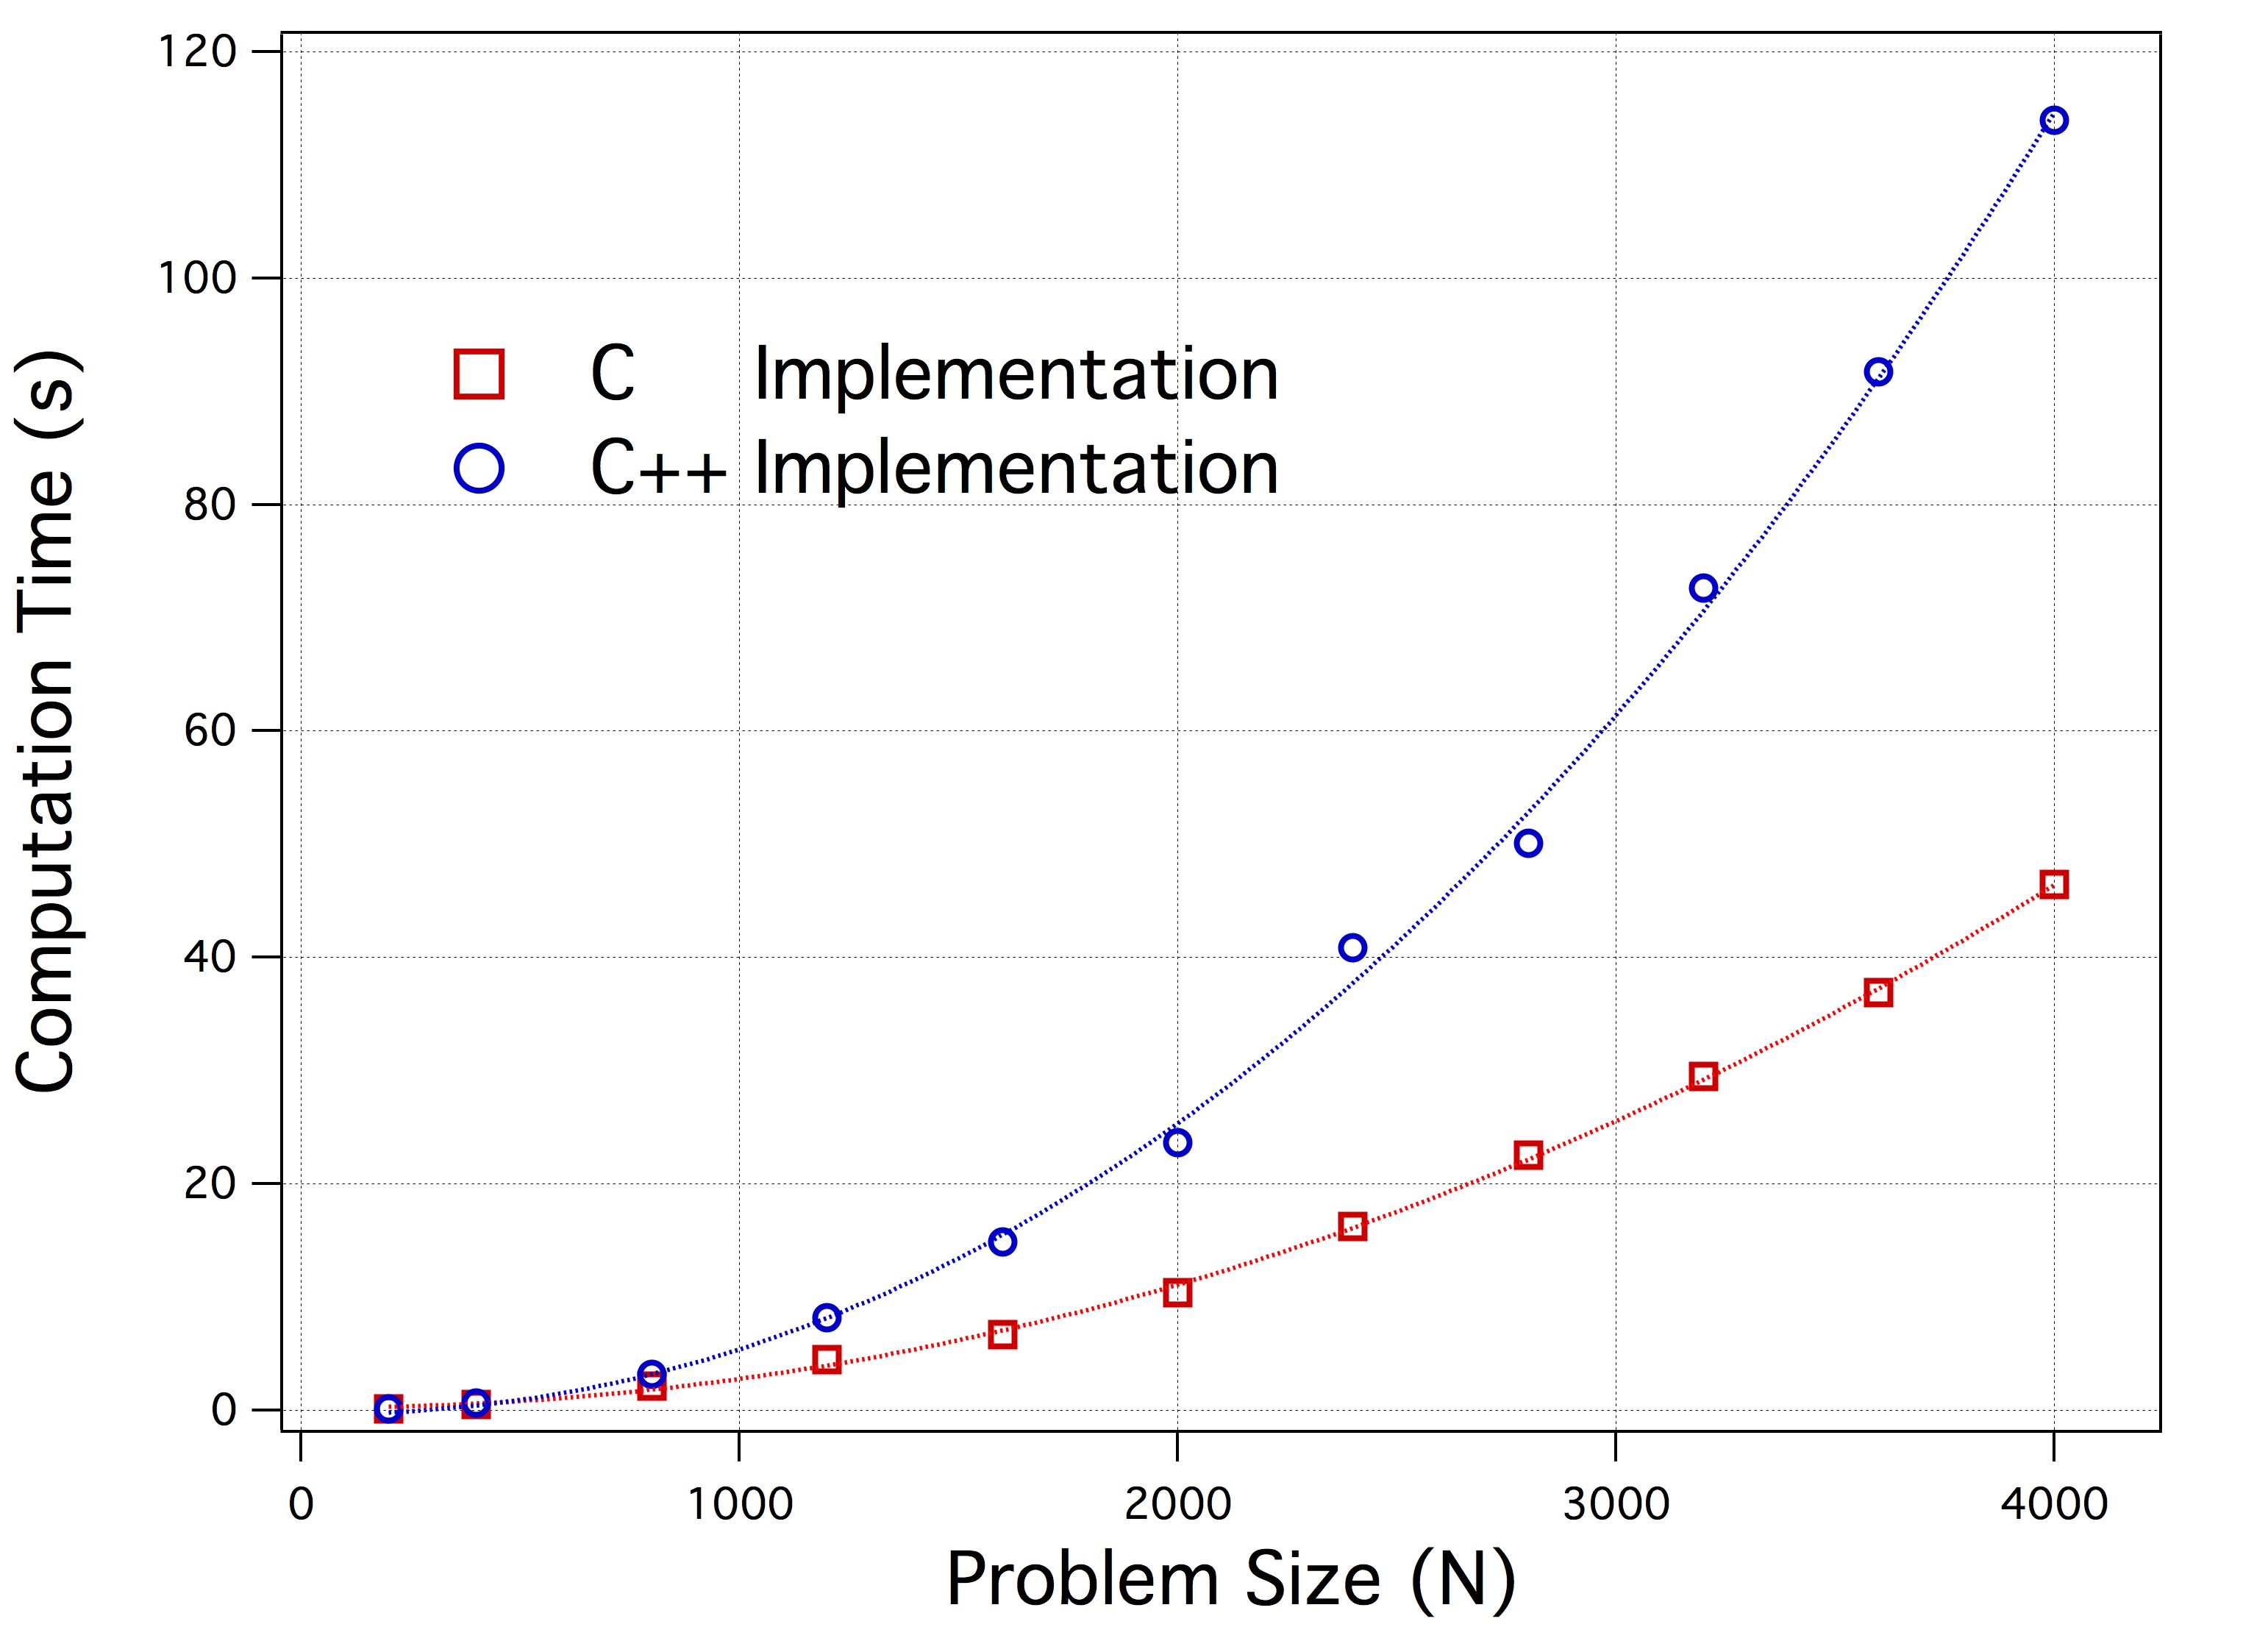
\includegraphics[width=0.5\textwidth]{performance.jpg}
                \caption {The performance comparison of C vs. C++ implementation (both serial and parallel). The thread number (16) is chosen so that the parallel code gets close nearly maximum performance.}
                \label{performance}
	\end{figure}
%	\begin{multicols}{2}
	For the serial code in figure(\ref{performance}), C++ implementation scales as $O(N^{2.16})$ and the C implementation scales as $O(N^{2.08})$. The coefficient comes from fitting the data with a power curve $y = y_0+Ax^{n}$. 
	\par For small problem size $N\sim100$, the C++ code runs faster possibly due to the fact that most of the data can fit into the cache memory. But the C implementation soon outperforms its counterpart as the problem size increases.
	\par For parallel code, the same thing happens. The C++ implementation takes only $0.058s$ for $N=200$ but the C version takes $0.30 s$ with the same condition. This overhead cost soon gets compensated by the speedup we get from better memory access and more cache-friendly operations.
	\subsection{Strong \& Weak Scaling}
%	\end{multicols}
	\begin{figure}[H]
        \centering
                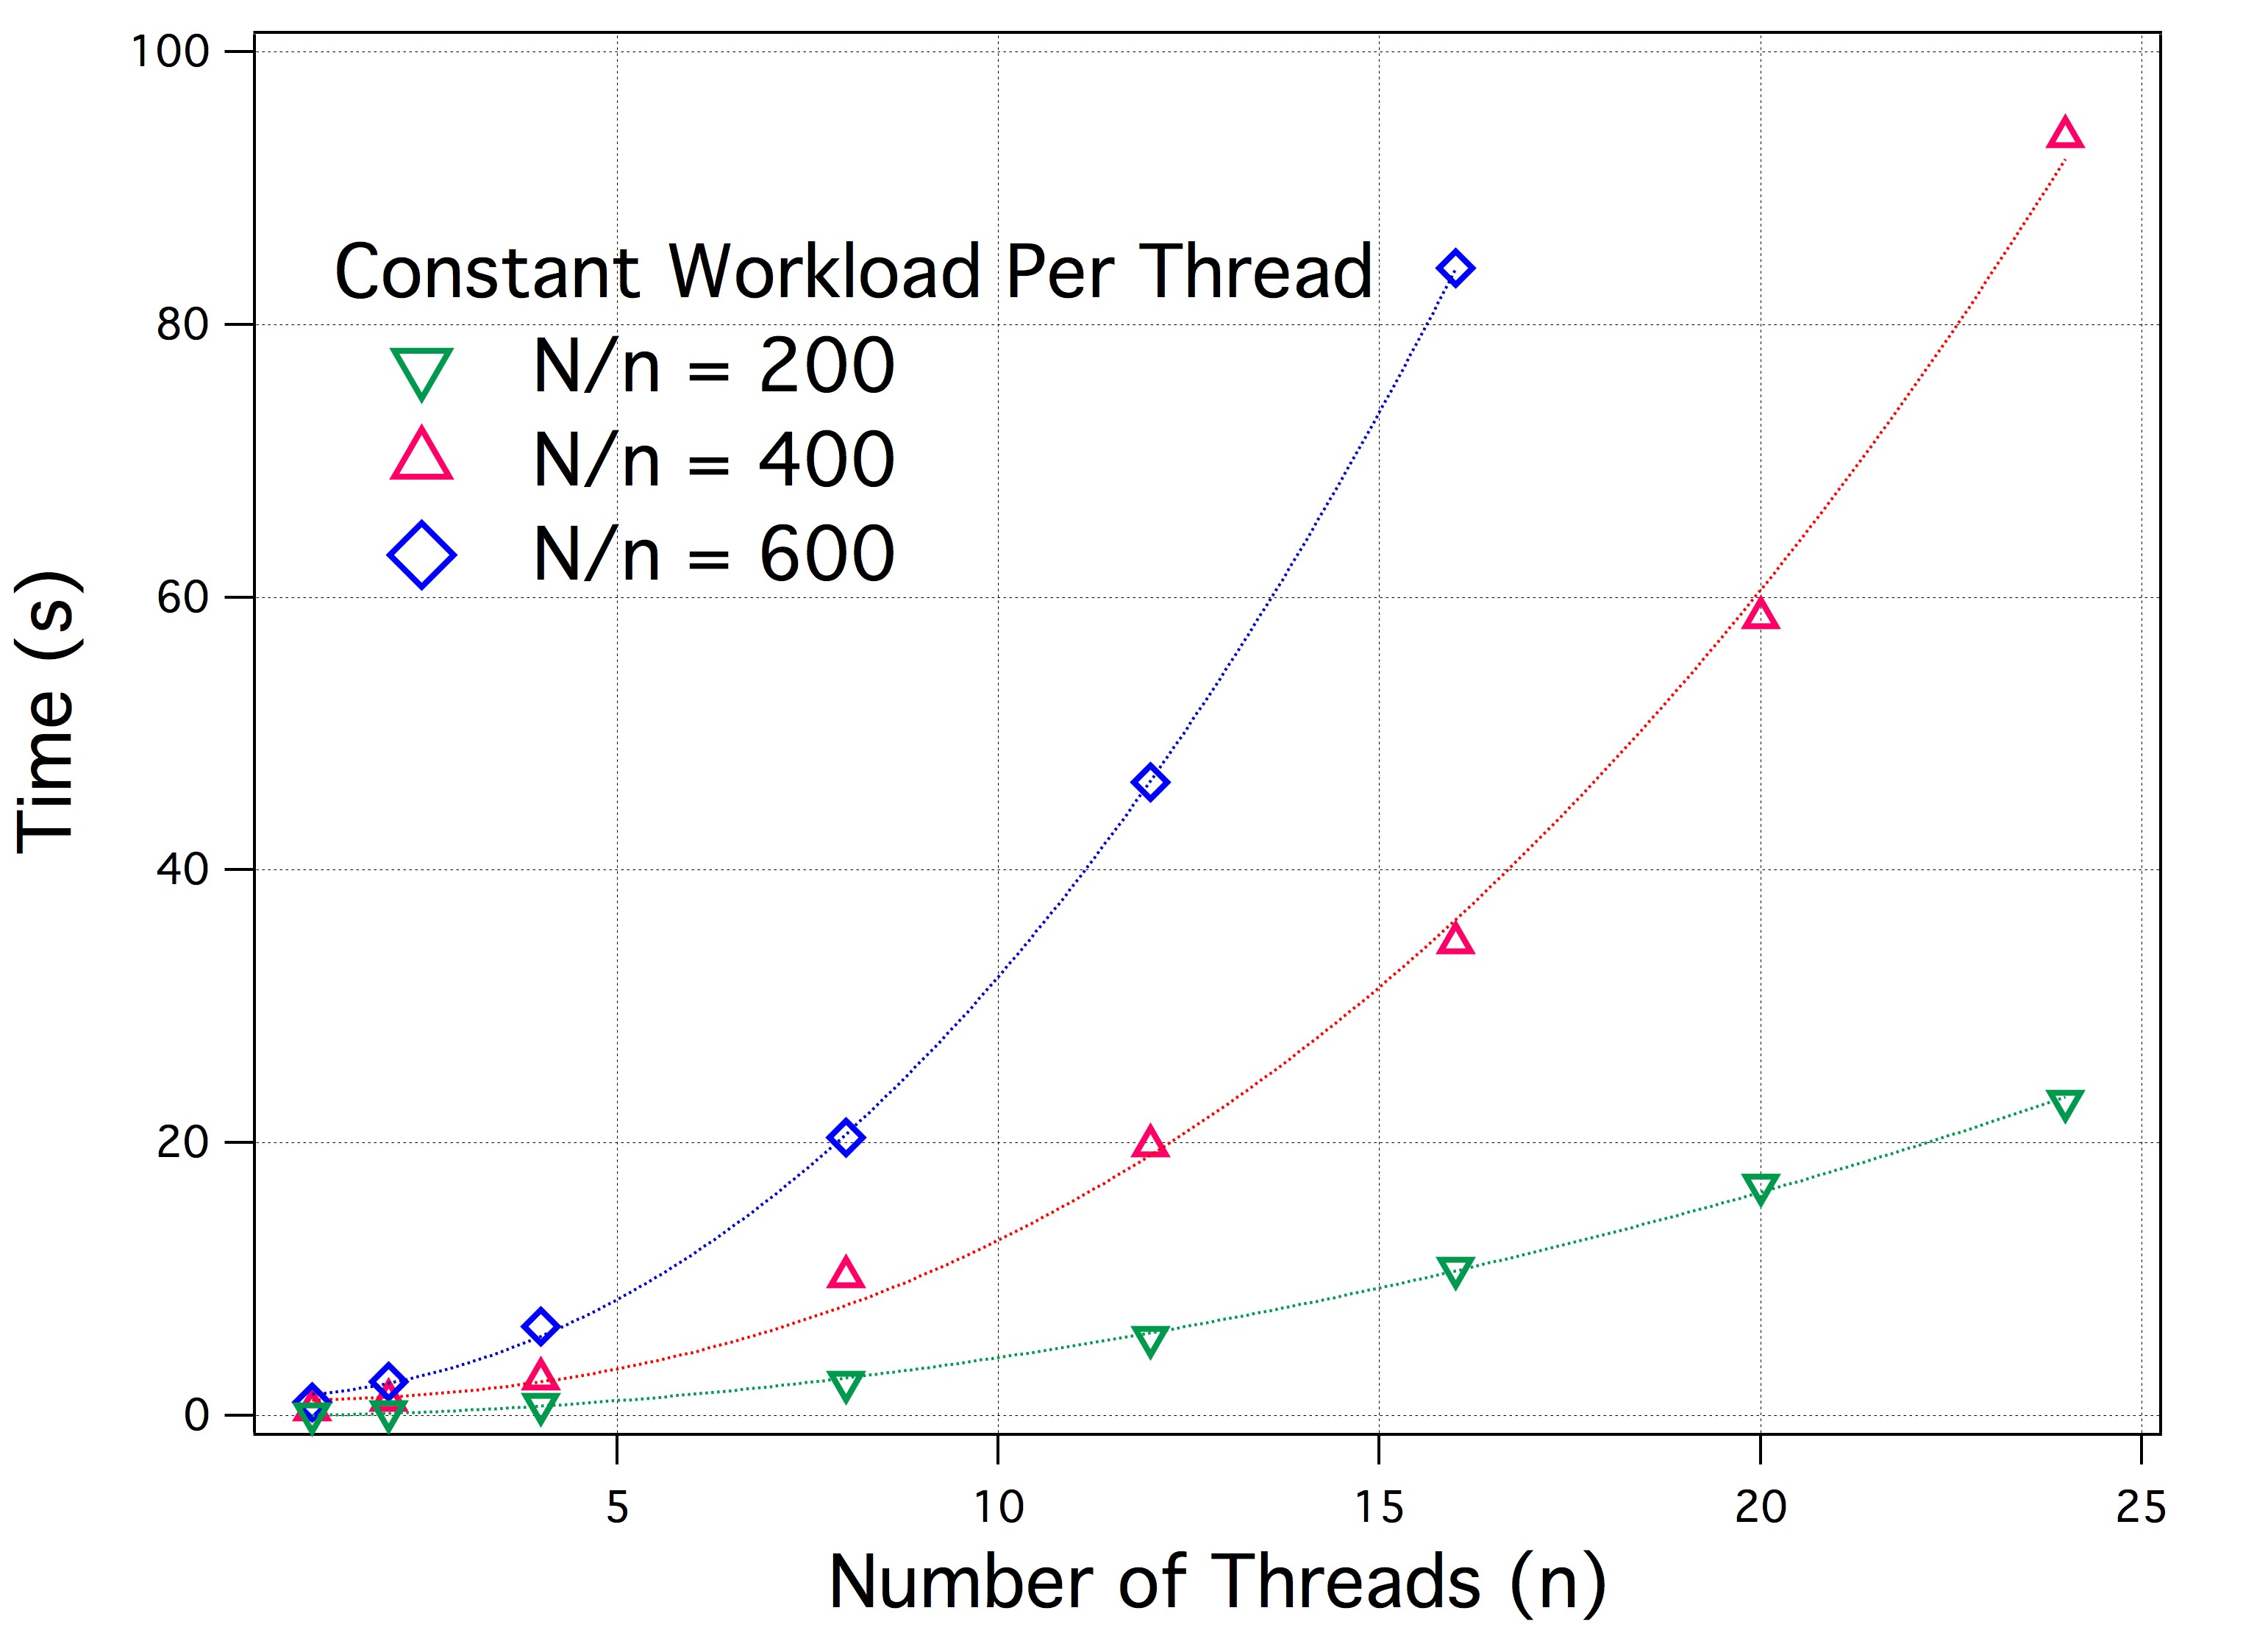
\includegraphics[width=0.5\textwidth]{weak_scaling.jpg}
                \caption {Weak scaling plot for C code with constant workload for each thread. Workloads are chosen to be $N/n = 200,~400, ~600$. Part of the $N/n = 600$ plot is missing because we exceeded the limit of available physical memory.}
                \label{weak}
	\end{figure}
%	\begin{multicols}{2}
	In figure(\ref{weak}), we are not achieving linear scaling because we only parallelize a fraction of our code. Besides, we have large overhead due to global communication patterns(transposing a matrix). 
%	\end{multicols}
	\begin{figure}[H]
        \centering
                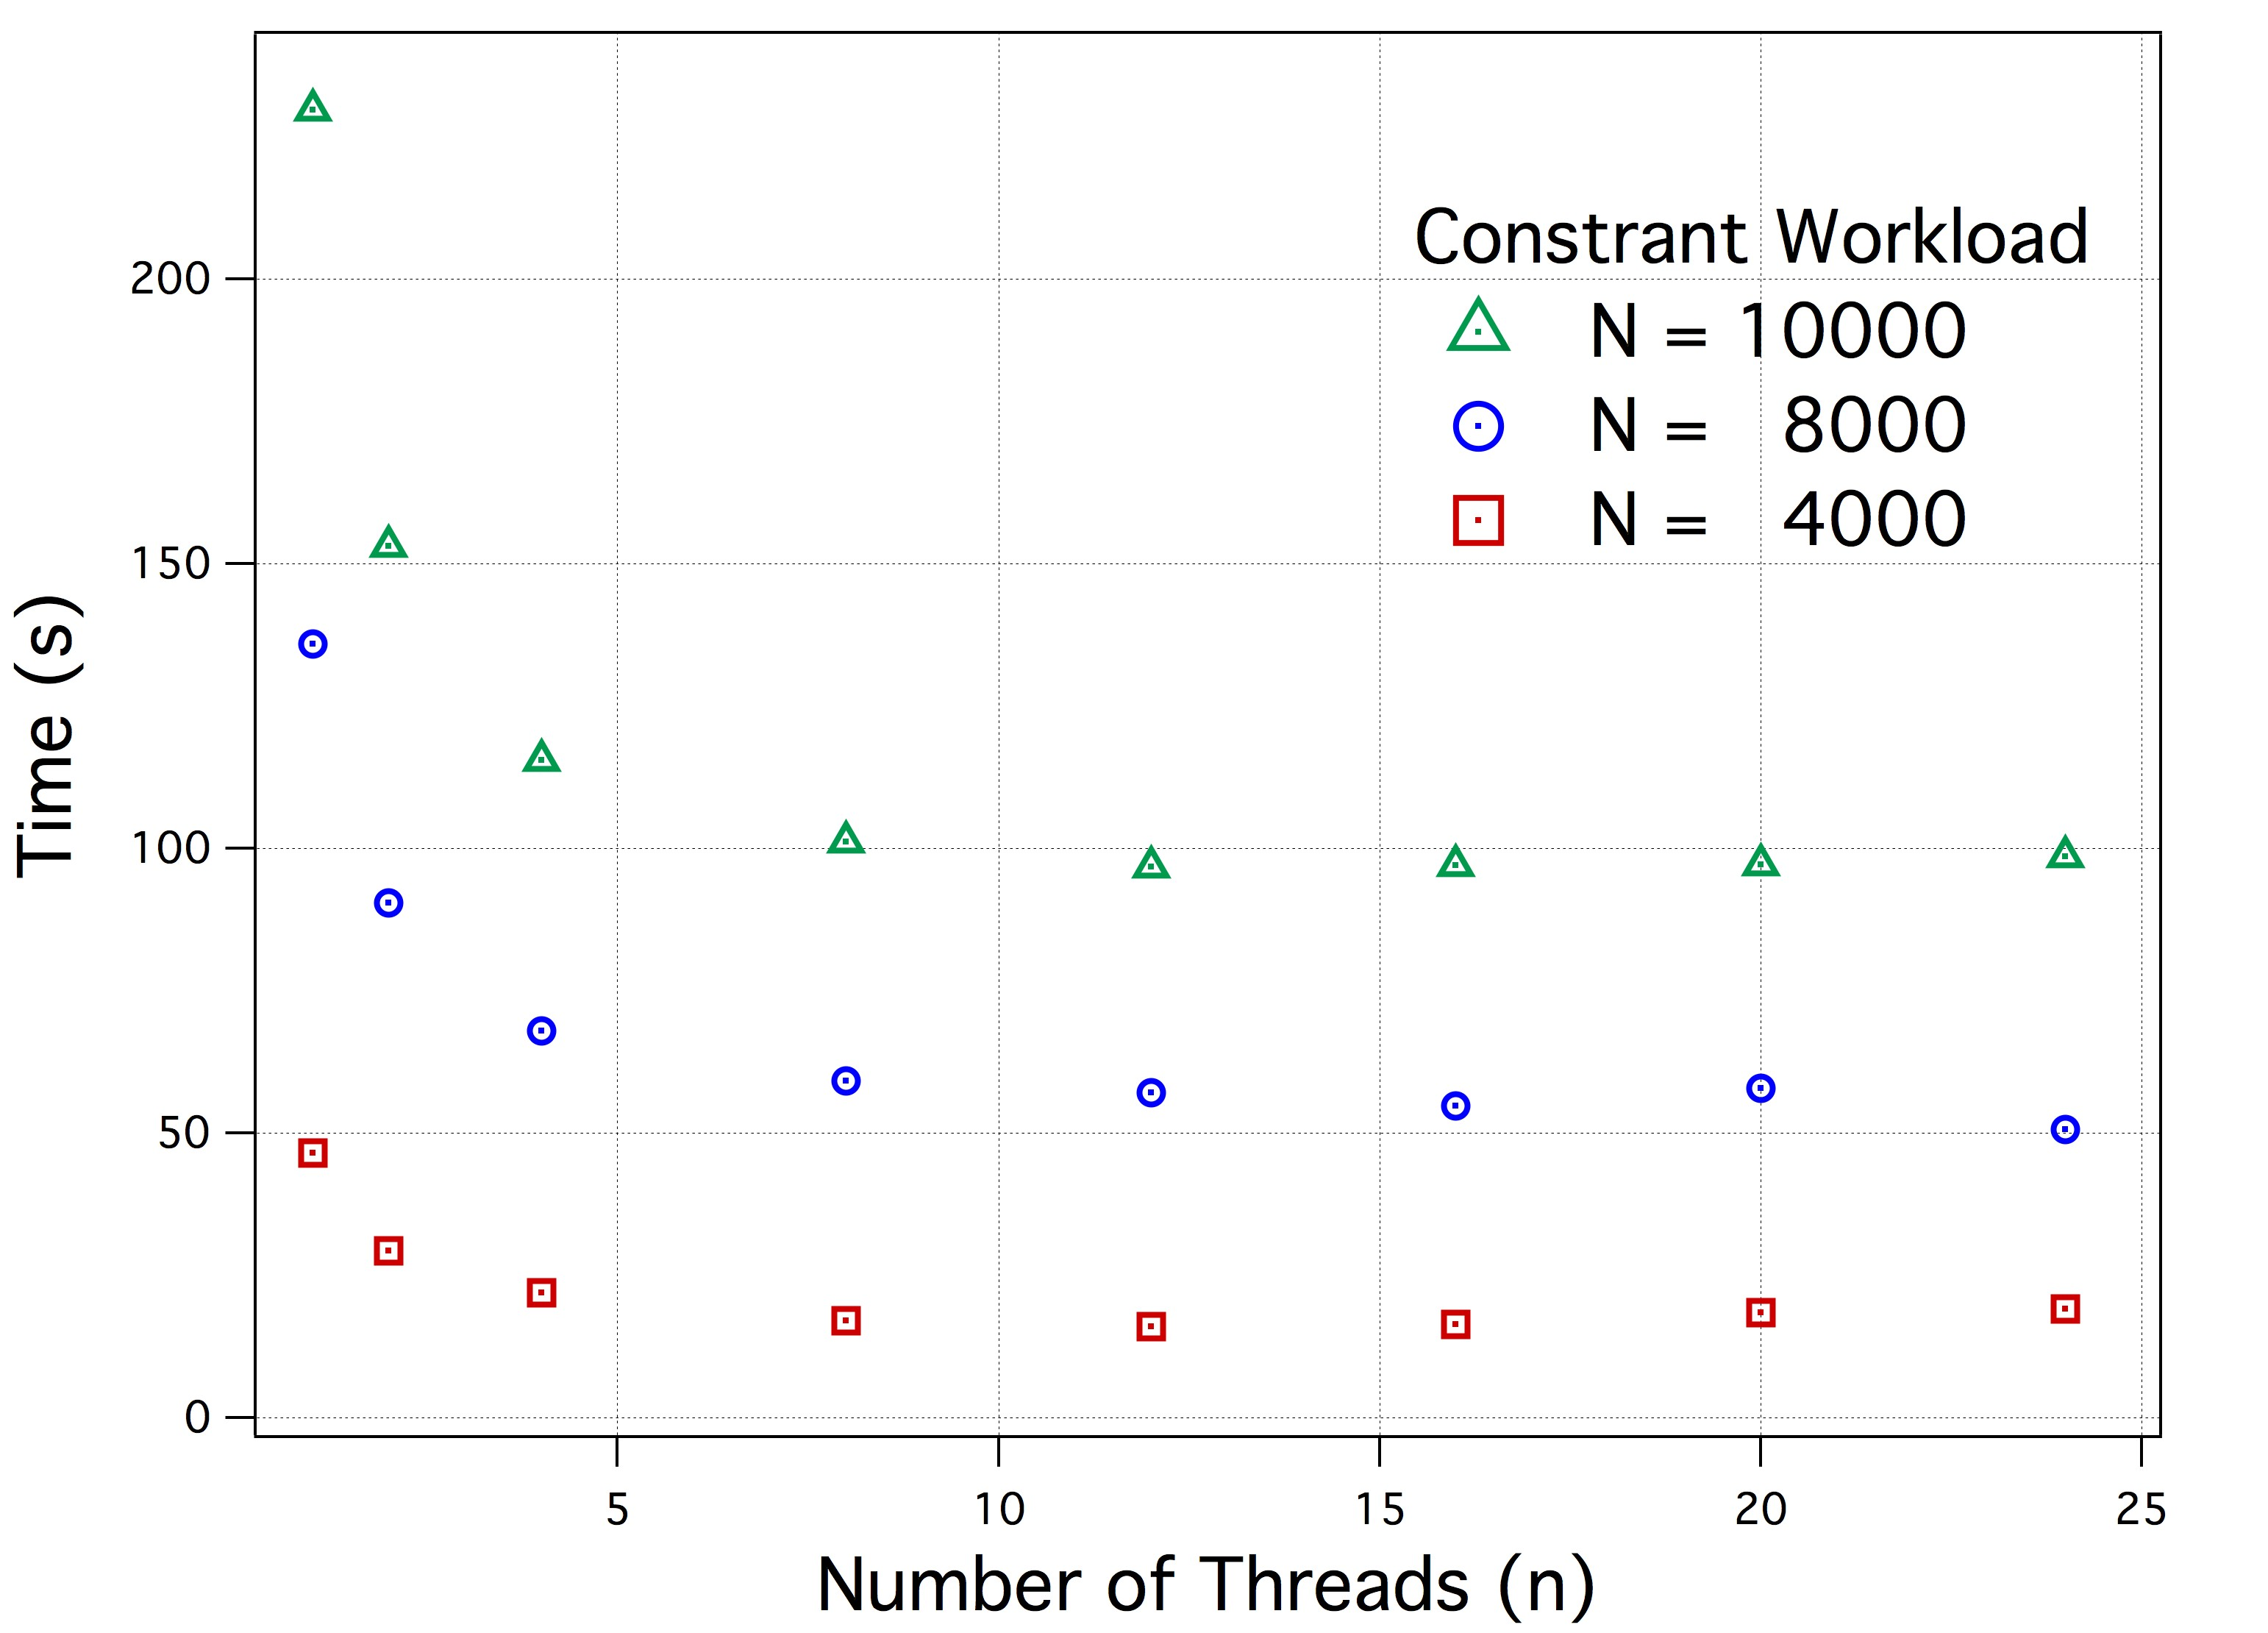
\includegraphics[width=0.5\textwidth]{strong_scaling.jpg}
                \caption {Strong scaling for C code with constant total workload. The total workloads are chosen to be $N = 4000,~8000,~10000$.}
                \label{strong}
	\end{figure}
	\begin{table}[H]
	\centering
	\label{my-label}
	\begin{tabular}{l|llllllll}
	\# of Threads   & 1     & 2     & 4     & 8     & 12    & 16    & 20    & 24    \\\hline
	Efficiency (\%) & 135.9 & 90.52 & 67.97 & 59.18 & 57.13 & 54.82 & 57.96 & 50.72
	\end{tabular}
	\caption{Strong scaling for C code for $N = 8000$ test case.}
	\end{table}
%	\begin{multicols}{2}
	In figure (\ref{strong}) and (\ref{efficiency}), we can see that the performance of parallel code only increases marginally when we use more than 8 threads. One explanation is that we are accessing the same aligned memory block for each computation and the performance is limited by the memory access speed instead of the computational speed.
%	\end{multicols}
	\begin{figure}[H]
        \centering
                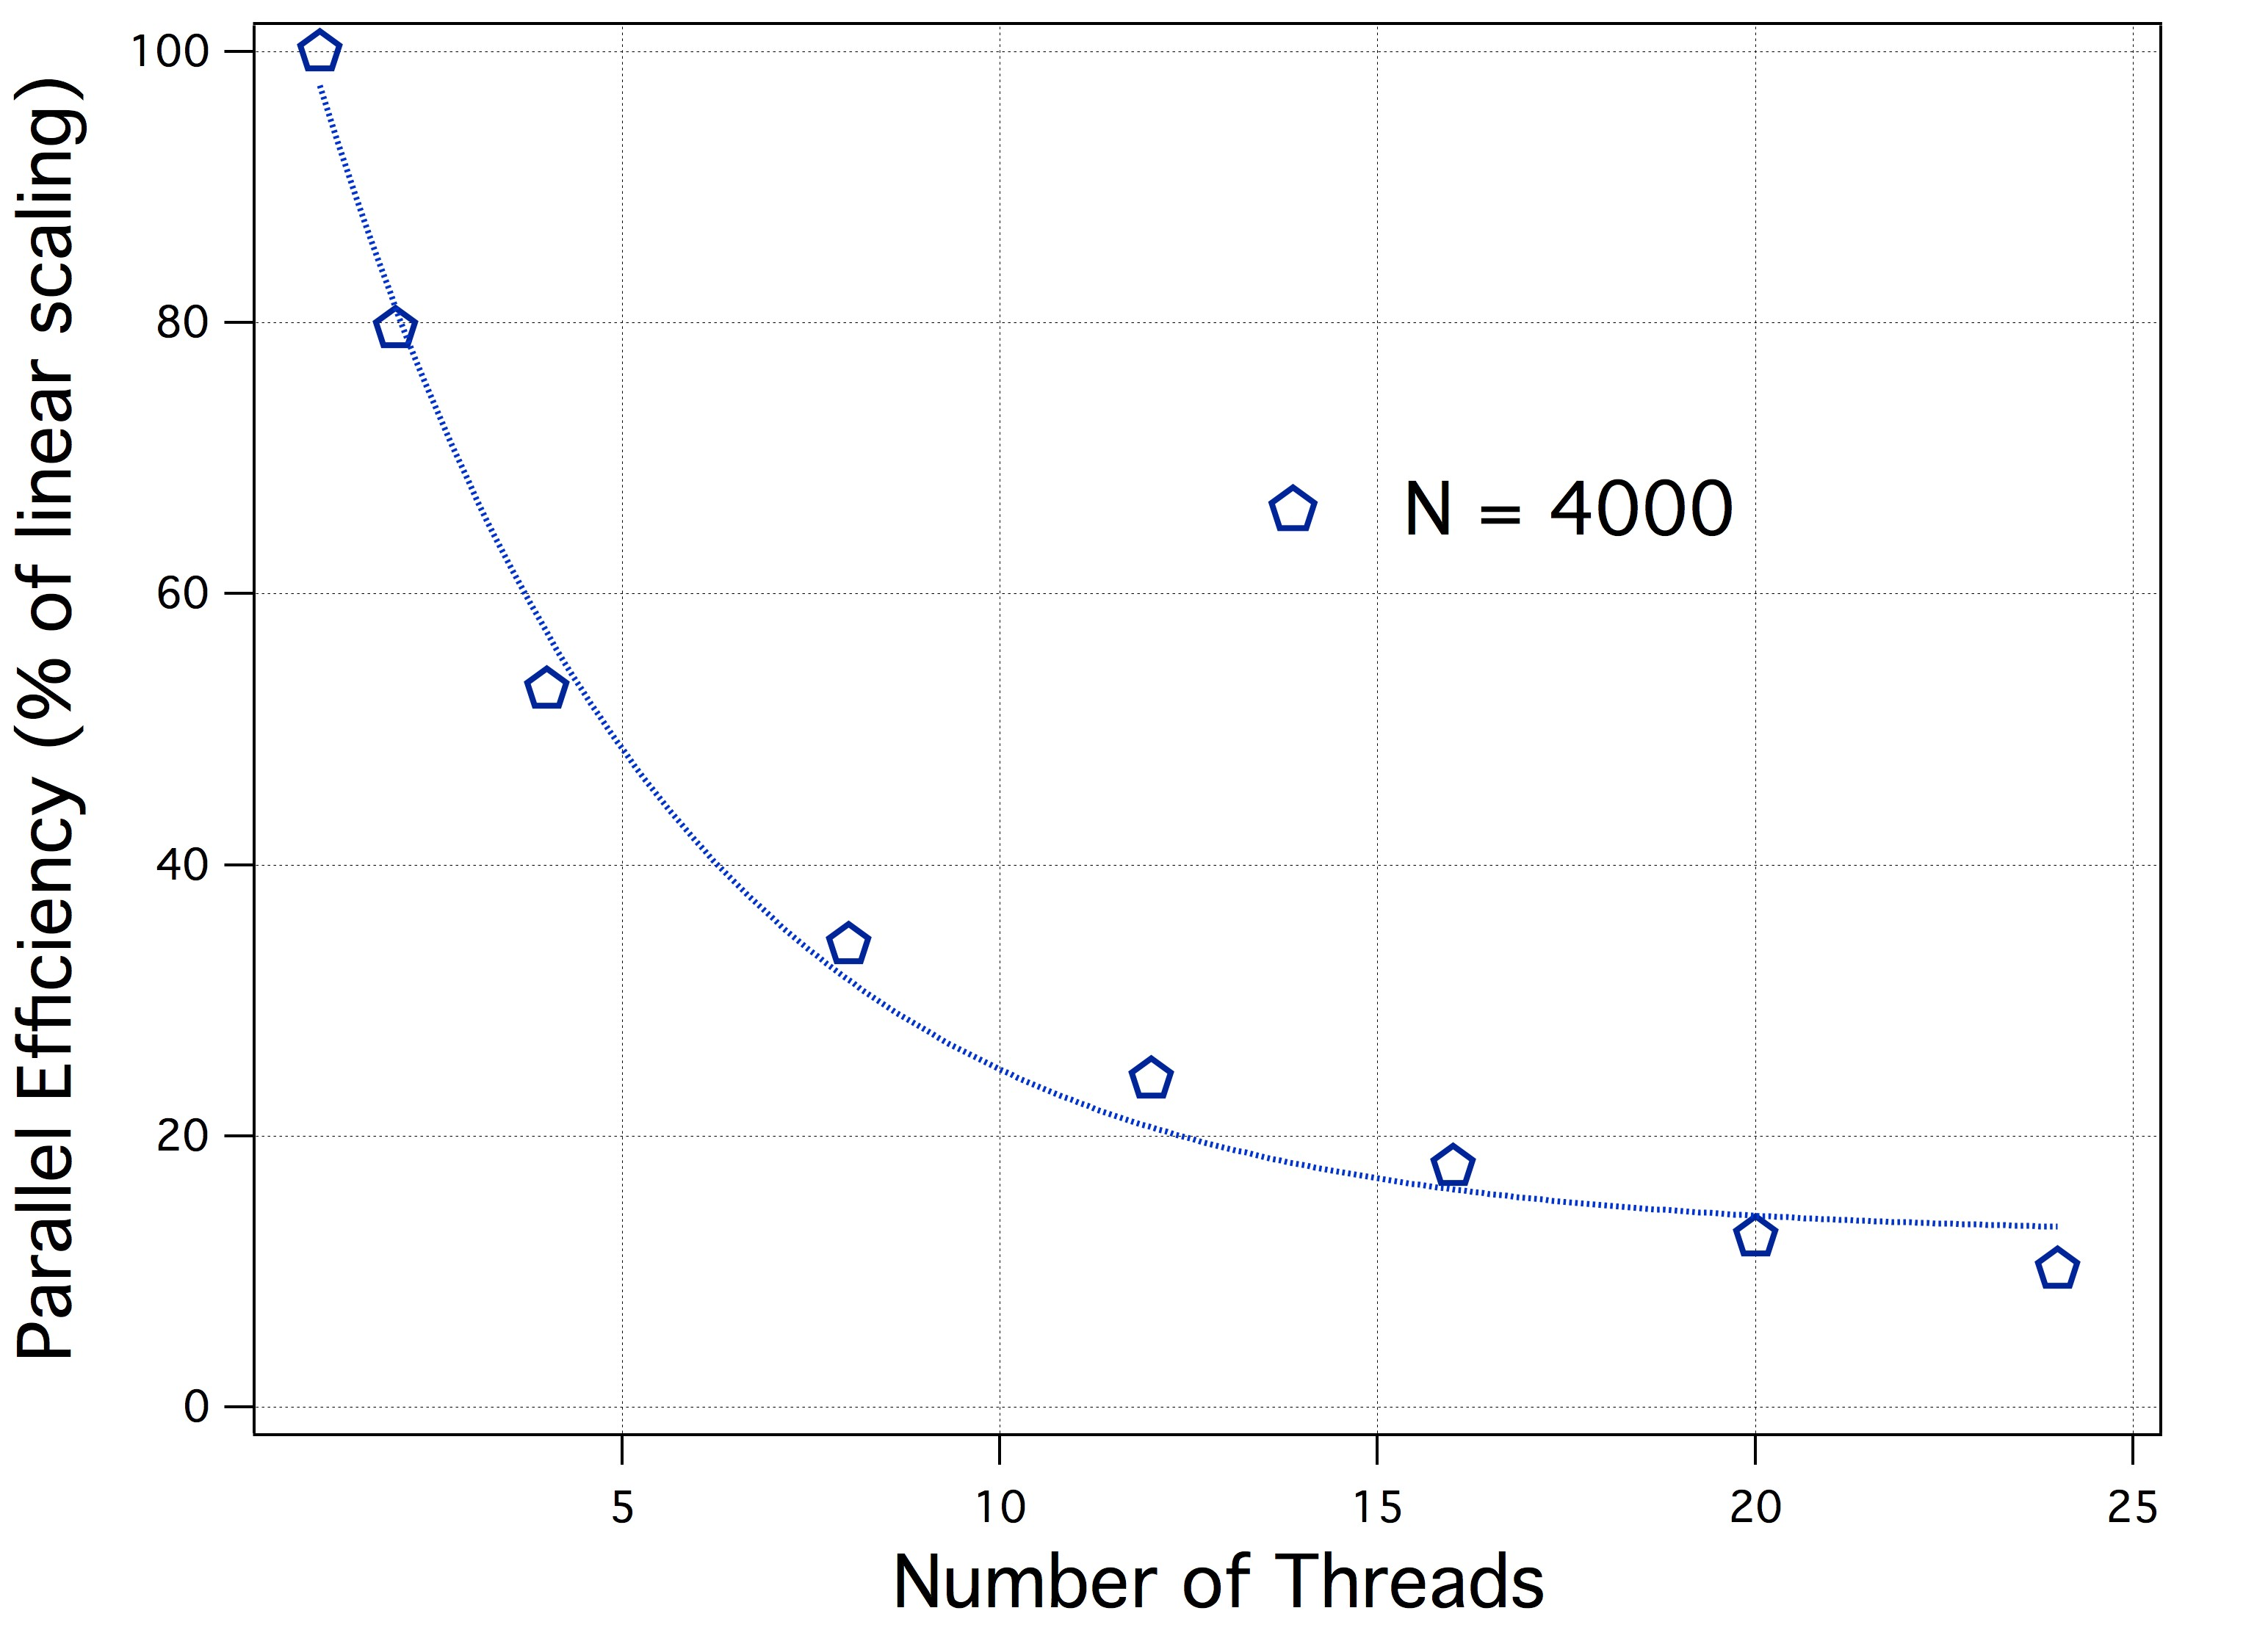
\includegraphics[width=0.5\textwidth]{efficiency.jpg}
                \caption {Parallel efficiency plot for $N = 4000$ case.}
                \label{efficiency}
	\end{figure}
	\begin{table}[H]
	\centering
	\label{my-label}
	\begin{tabular}{l|llllllll}
	\# of Threads   & 1   & 2     & 4     & 8     & 12    & 16    & 20    & 24    \\
	\hline
	Efficiency (\%) & 100 & 79.57 & 53.00 & 34.15 & 24.19 & 17.76 & 12.59 & 10.17
	\end{tabular}
	\caption{Parallel Efficiency Plot for $N = 4000$ test case.}
	\end{table}
	\begin{multicols}{2}
\section{Discussion}
	\subsection{Results}
	We identified the bottlenecks of our reference code and tried to improve its serial performance. Later we rewrote the code in C for finer control over the memory access and vectorization. We chose a data structure that is efficienct for most computation and transposed the matrix only when it became necessary. We also added difference norm check to stop our iteration sooner at the cost of extra \verb|normInf()| computation and data update.
	\par As a result, we have a more controlled memory access flow and we have vectorized the computation in our relaxation operation. We achieved good performance improvement for both serial and parallel implementation. For problem size $N = 2000$, the serial code runs more than twice faster.
	\par After that, we parallelized our code for further speedup. We chose parallel sections sparingly to avoid the overhead cost to launch thread teams. In the end, we limit our parallel work to the most computationally intense part - backsolving the 1D tridiagonal linear systems. The nature of our algorithm makes it easy for us to parallelize the code using OpenMP and see an improvement on the serial code.
	\par Despite the ease to incoporate OpenMP in our code, it proves difficult to make the parallization more efficient. We tried various techniques to reduce the serial work between two \verb|omp parallel for| loops and balance workload for each thread. After experimenting with different instructions, we used \verb|schedule(dynamic, 8)| to get the best performance of our parallel code.
	\subsection{What else could be done}
	As we discussed in weak/strong scaling section, the parallel code performance is limited by memory access speed when we are using more than $8$ threads. One way we can address this problem is to divide the memory block and store our data in several subblocks for each thread. In this case, MPI may be a better choice because each thread will keep their own copy and they only communicate when necessary. The challenge is to address the global communication pattern that we have for the Douglas ADI method. It is inevitable to transpose our matrices and switch the direction of our backsolver, so a more sophisticated data structure and communication strategy are needed for that to happen.
	\par The other approach to improving the program is to increase the arithmetic intensity of our computation. The Douglas ADI method has the advantage of reducing multidimensional problem to a series of simpler 1D problems, but this limits our ability to write arithematically intense code from a computational perspective. If we can rewrite the math algorithm in a way such that matrix tranpose can be done implicitly, we can pack the other operations into our parallel section and increase the intensity.
	\par Lastly, we suggest using LAPACK or other linear algebra library to carry out some of the operations. As obvious in project 1, the optimized libraries can do a much better job than our honest attempts. In our case, it is not clear if we can see a significant boost in the speed because we are using Thomas algorithm and it is by a nature a simple algorithm and hard to improve. However, it will be interesting to see what difference that can make.
\end{multicols}

\newpage
\begin{thebibliography}{9}
\bibitem{A Note on the Alternating Direction Implicit Method for the Numerical Solution of Heat Flow Problems} 
 Douglas, Jim. 
\textit{A Note on the Alternating Direction Implicit Method for the Numerical Solution of Heat Flow Problems}. 
roceedings of the American Mathematical Society 8.2 (1957): 409 -- 412. 

\bibitem{book} 
 Strikwerda, John C. 
 "The Alternating Direction Implicit Method."
\textit{Finite Difference Schemes and Partial Differential Equations}. 2nd ed. Pacific Grove, CA: Wadsworth \& Brooks/Cole Advanced Software, 1989.
 
\bibitem{knuthwebsite} 
Chang, M. J., L. C. Chow, and W. S. Chang. 
\textit{Improved Alternating-Direction Implicit Method For Solving Transient Three-Dimensional Heat Diffusion Problems.} Numerical Heat Transfer, Part B: Fundamentals: 69-84.
\end{thebibliography}

\end{document}
